\documentclass[a4paper,11pt]{scrartcl}
\usepackage[margin=0.3in]{geometry}
\usepackage{graphicx}
\usepackage{textcomp}
\usepackage{subcaption}
\usepackage{array}
\usepackage{listings}
\usepackage[colorlinks=true, citecolor=black, linkcolor=black, urlcolor=black, bookmarks]{hyperref}
\usepackage{color}

\definecolor{mygreen}{rgb}{0,0.6,0}
\definecolor{mygray}{rgb}{0.5,0.5,0.5}
\definecolor{mymauve}{rgb}{0.58,0,0.82}

\lstset{ %
  backgroundcolor=\color{white},   % choose the background color; you must add \usepackage{color} or \usepackage{xcolor}
  basicstyle=\footnotesize,        % the size of the fonts that are used for the code
  breakatwhitespace=false,         % sets if automatic breaks should only happen at whitespace
  breaklines=true,                 % sets automatic line breaking
  captionpos=b,                    % sets the caption-position to bottom
  commentstyle=\color{mygreen},    % comment style
  deletekeywords={...},            % if you want to delete keywords from the given language
  escapeinside={\%*}{*)},          % if you want to add LaTeX within your code
  extendedchars=true,              % lets you use non-ASCII characters; for 8-bits encodings only, does not work with UTF-8
  frame=single,                    % adds a frame around the code
  keepspaces=true,                 % keeps spaces in text, useful for keeping indentation of code (possibly needs columns=flexible)
  keywordstyle=\color{blue},       % keyword style
  language=Bash,                 % the language of the code
  morekeywords={*,...},            % if you want to add more keywords to the set
  numbers=left,                    % where to put the line-numbers; possible values are (none, left, right)
  numbersep=5pt,                   % how far the line-numbers are from the code
  numberstyle=\tiny\color{mygray}, % the style that is used for the line-numbers
  rulecolor=\color{black},         % if not set, the frame-color may be changed on line-breaks within not-black text (e.g. comments (green here))
  showspaces=false,                % show spaces everywhere adding particular underscores; it overrides 'showstringspaces'
  showstringspaces=false,          % underline spaces within strings only
  showtabs=false,                  % show tabs within strings adding particular underscores
  stepnumber=1,                    % the step between two line-numbers. If it's 1, each line will be numbered
  stringstyle=\color{mymauve},     % string literal style
  tabsize=4,                       % sets default tabsize to 2 spaces
  title=\lstname                   % show the filename of files included with \lstinputlisting; also try caption instead of title
}

\begin{document}

\title{User Guide}
\subtitle{Radio Frequency Localisation of RFID Tags in a Raspberry-Pi Sensor Network}
\date{\today}
\author{Aleksandar Krastev (s0833784) \\ s0833784@sms.ed.ac.uk \\ sandio.mama@gmail.com}
\maketitle


\section{Hardware}

\begin{itemize}
	\item \textbf{3 x Raspberry Pi computers} (Raspberry Pi Type B Single Board Computer 512MB)\footnote{The Raspberry Pi website - \url{http://www.raspberrypi.org/faqs}.}
	\item \textbf{3 x RFID readers} (RF9315R-u Active RFID 8 Meters Receiver with RSSI Module)\footnote{Ananiah Electronics active RFID reader - \url{http://www.ananiahelectronics.com/RF9315R-u.htm}.}
	\item \textbf{1 x RFID tag} (RF8315T Active RFID 8 Meters Transmitting Module)\footnote{Ananiah Electronics active RFID tag - \url{http://www.ananiahelectronics.com/RF8315T.htm}.}
	\item \textbf{3 x SD cards} (SanDisk 4GB SDHC Secure Digital Card)	
	\item \textbf{3 x Power supplies} (UK 5V @ 1.2A power supply with integral 1.5m cable and micro-USB plug)
\end{itemize}

\begin{figure}[h]
	\centering
	\begin{subfigure}[b]{0.3\textwidth}
		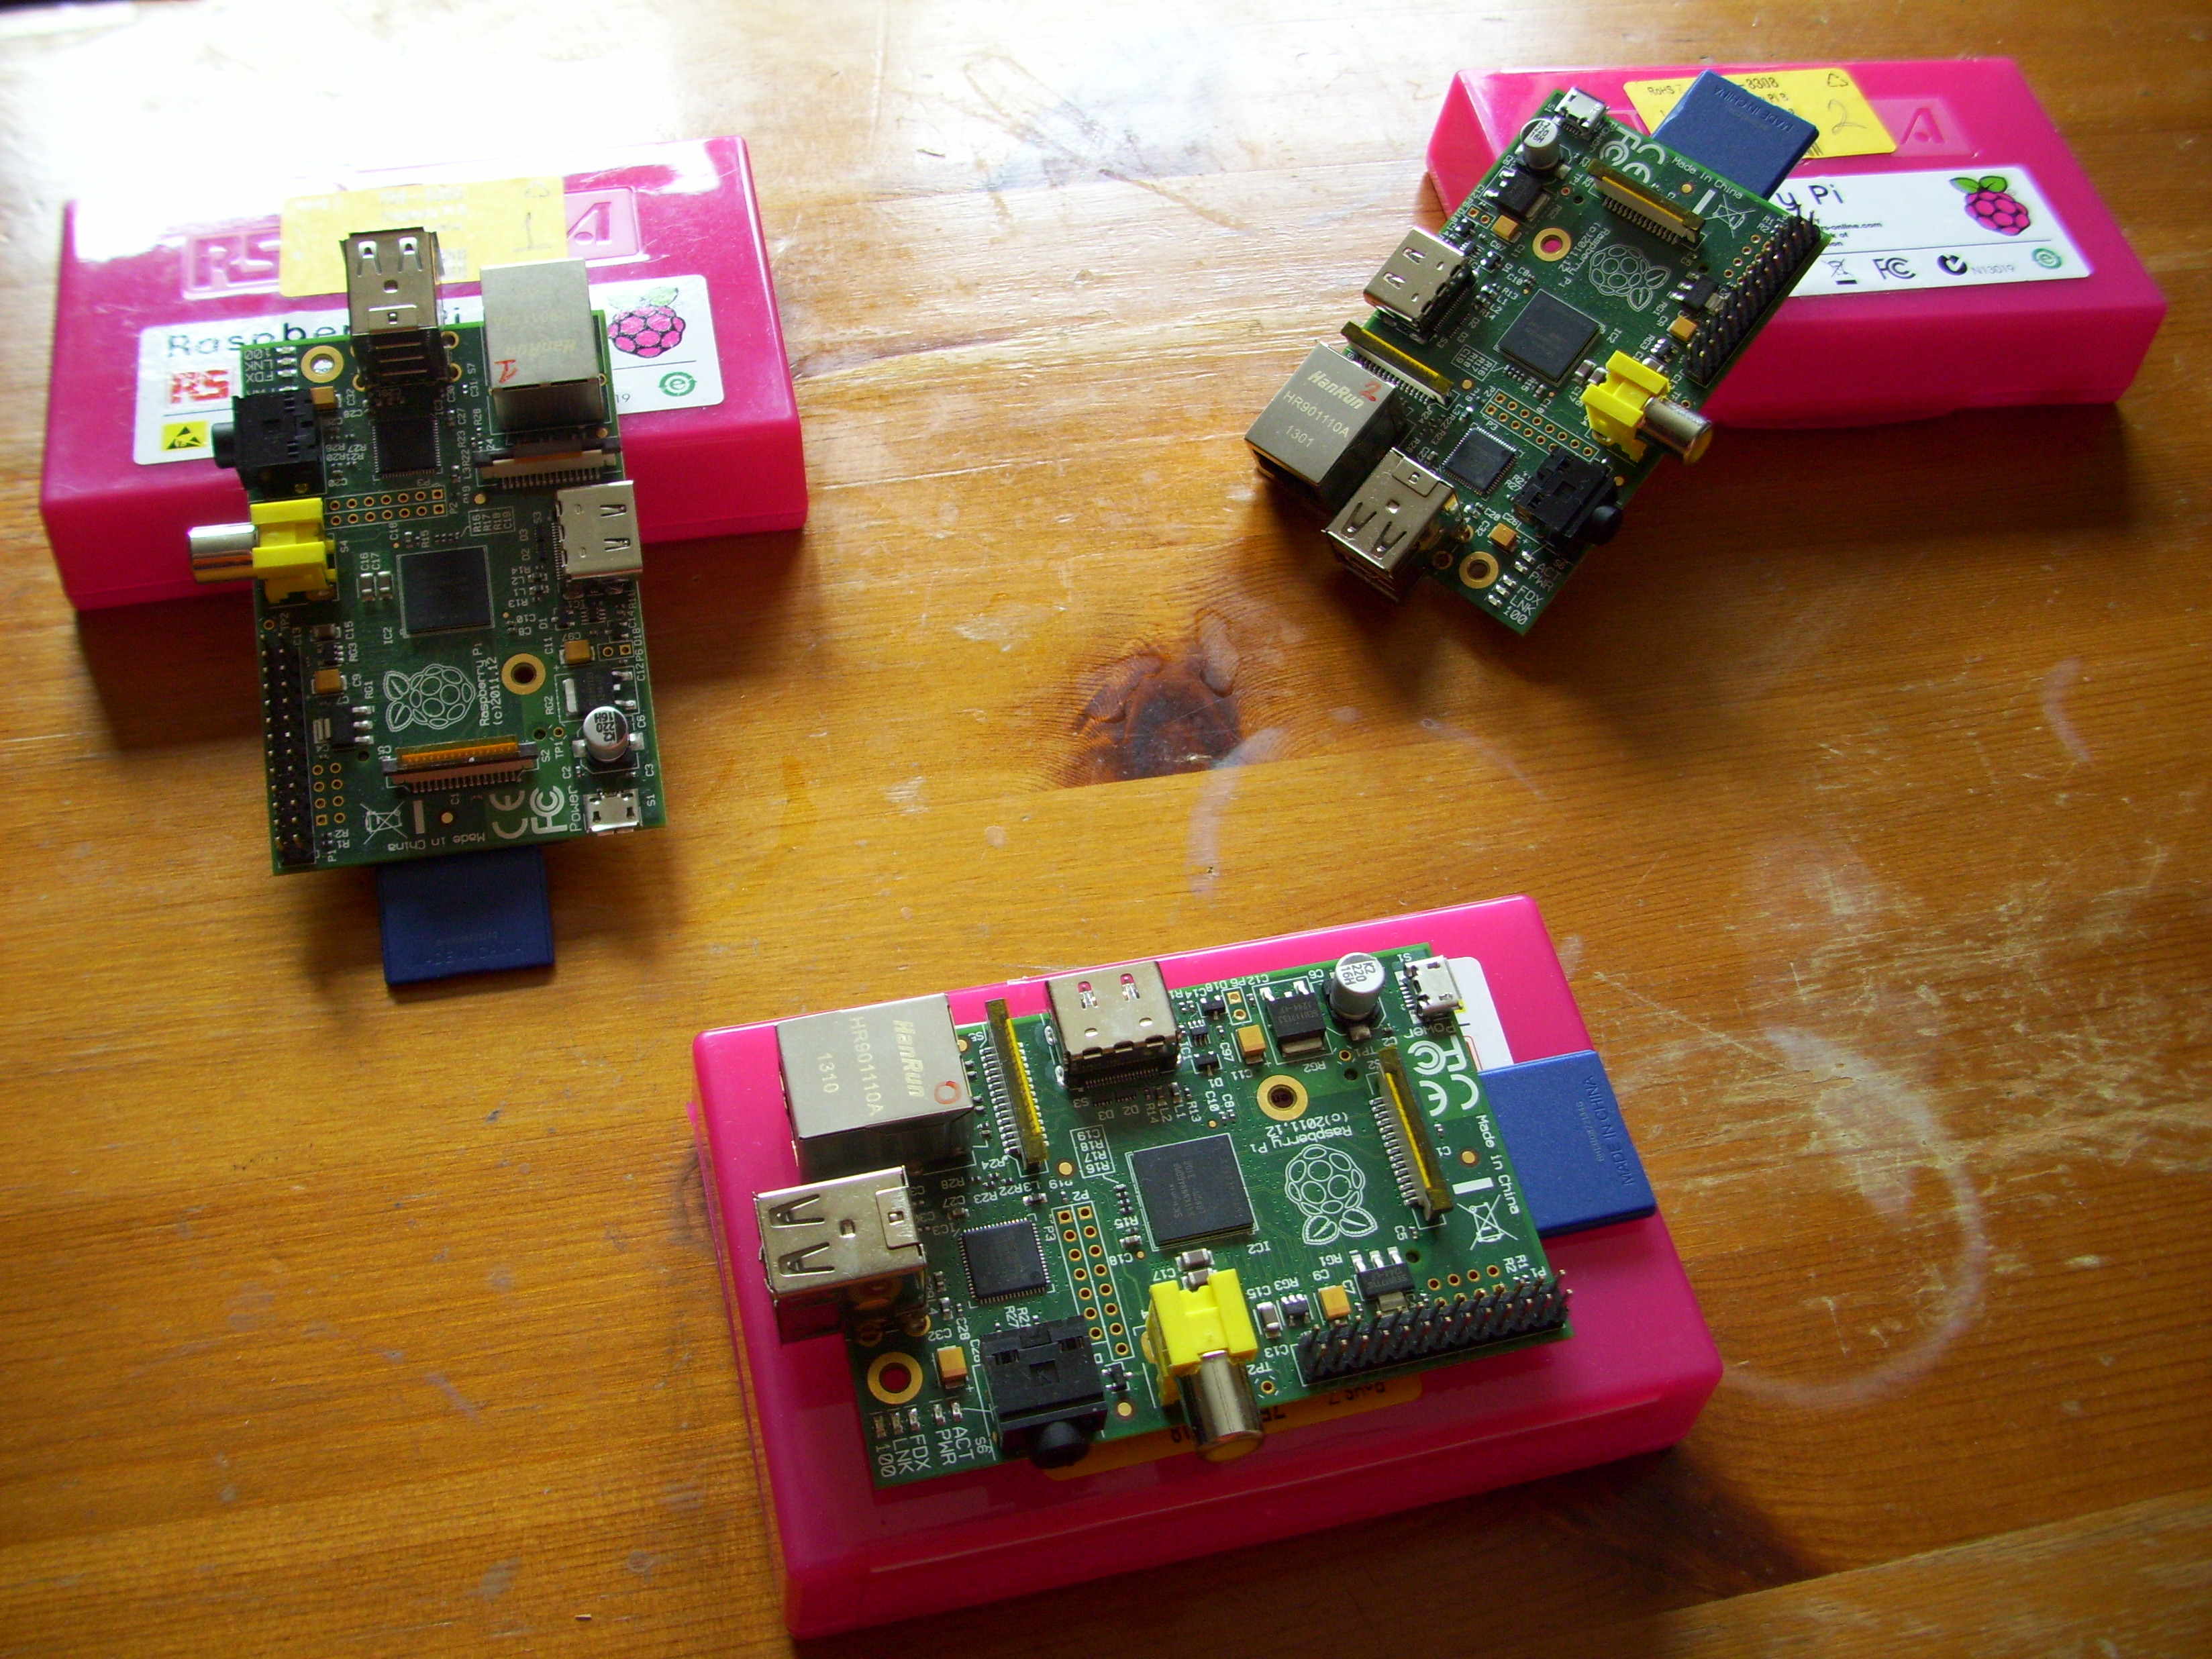
\includegraphics[width=\textwidth]{pis}
		\caption{Three Raspberry Pis}
	\end{subfigure}
	\begin{subfigure}[b]{0.3\textwidth}
		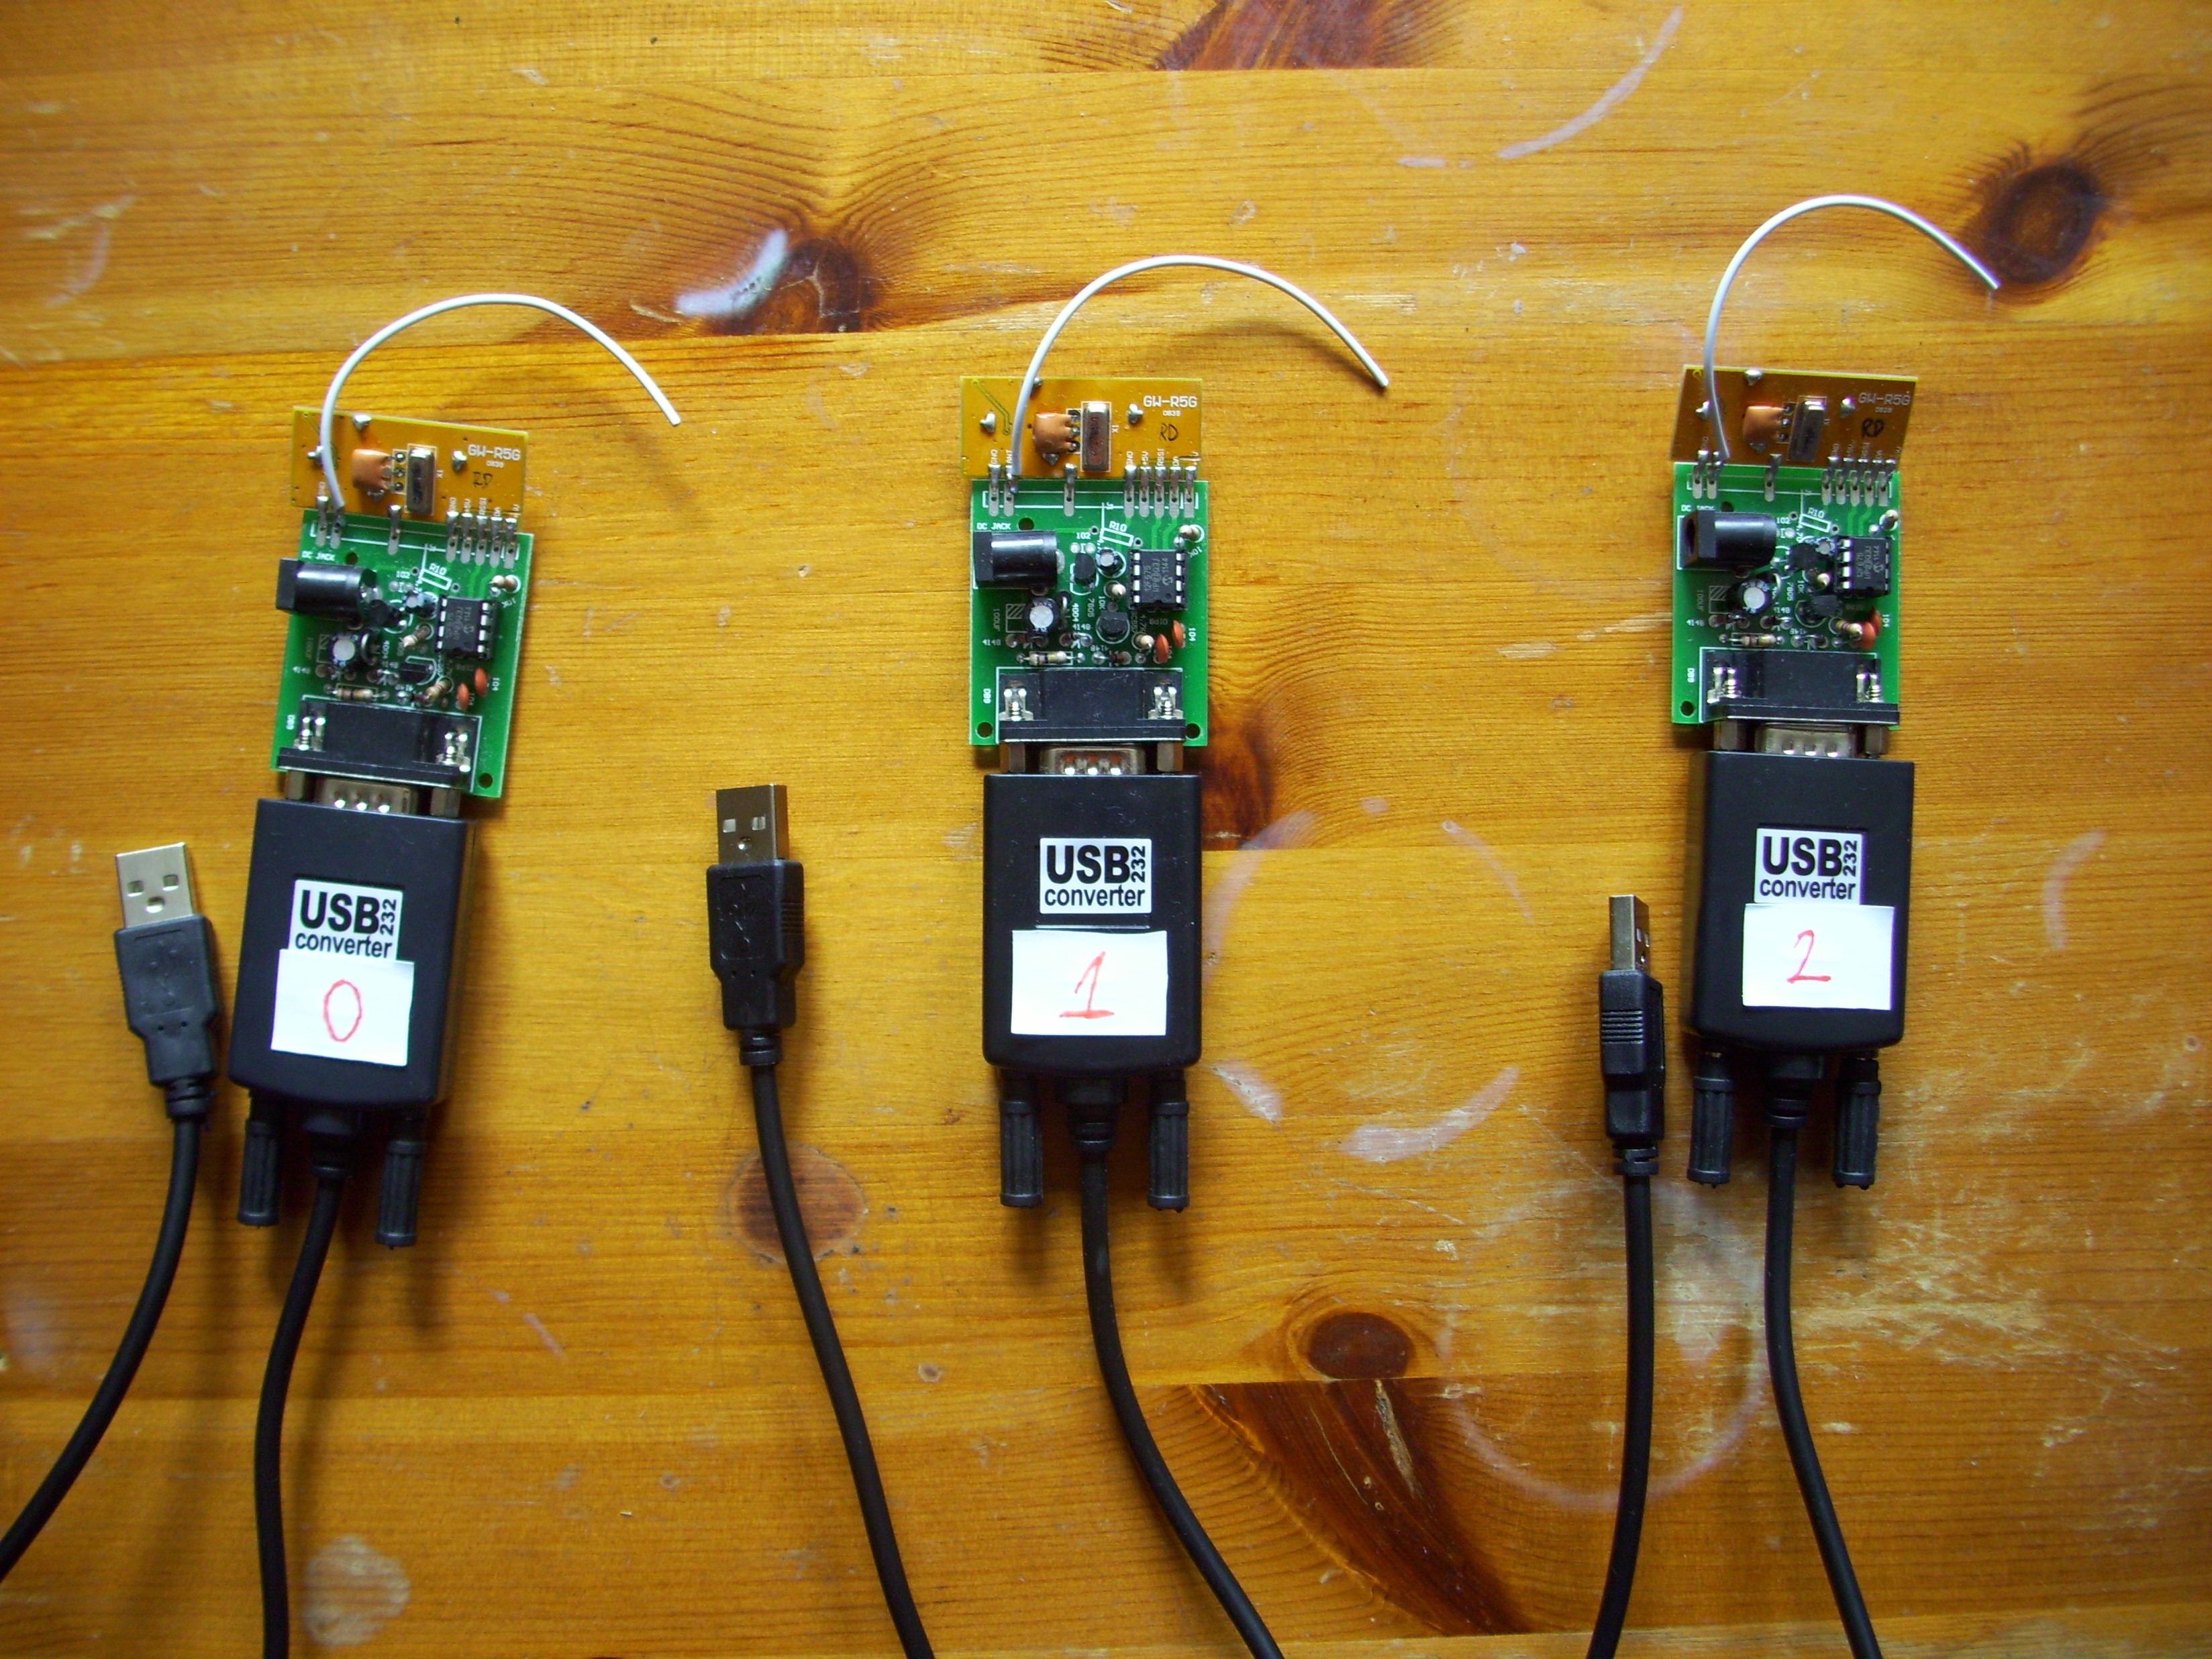
\includegraphics[width=\textwidth]{readers}
		\caption{Three active RFID readers}
	\end{subfigure}
	\begin{subfigure}[b]{0.3\textwidth}
		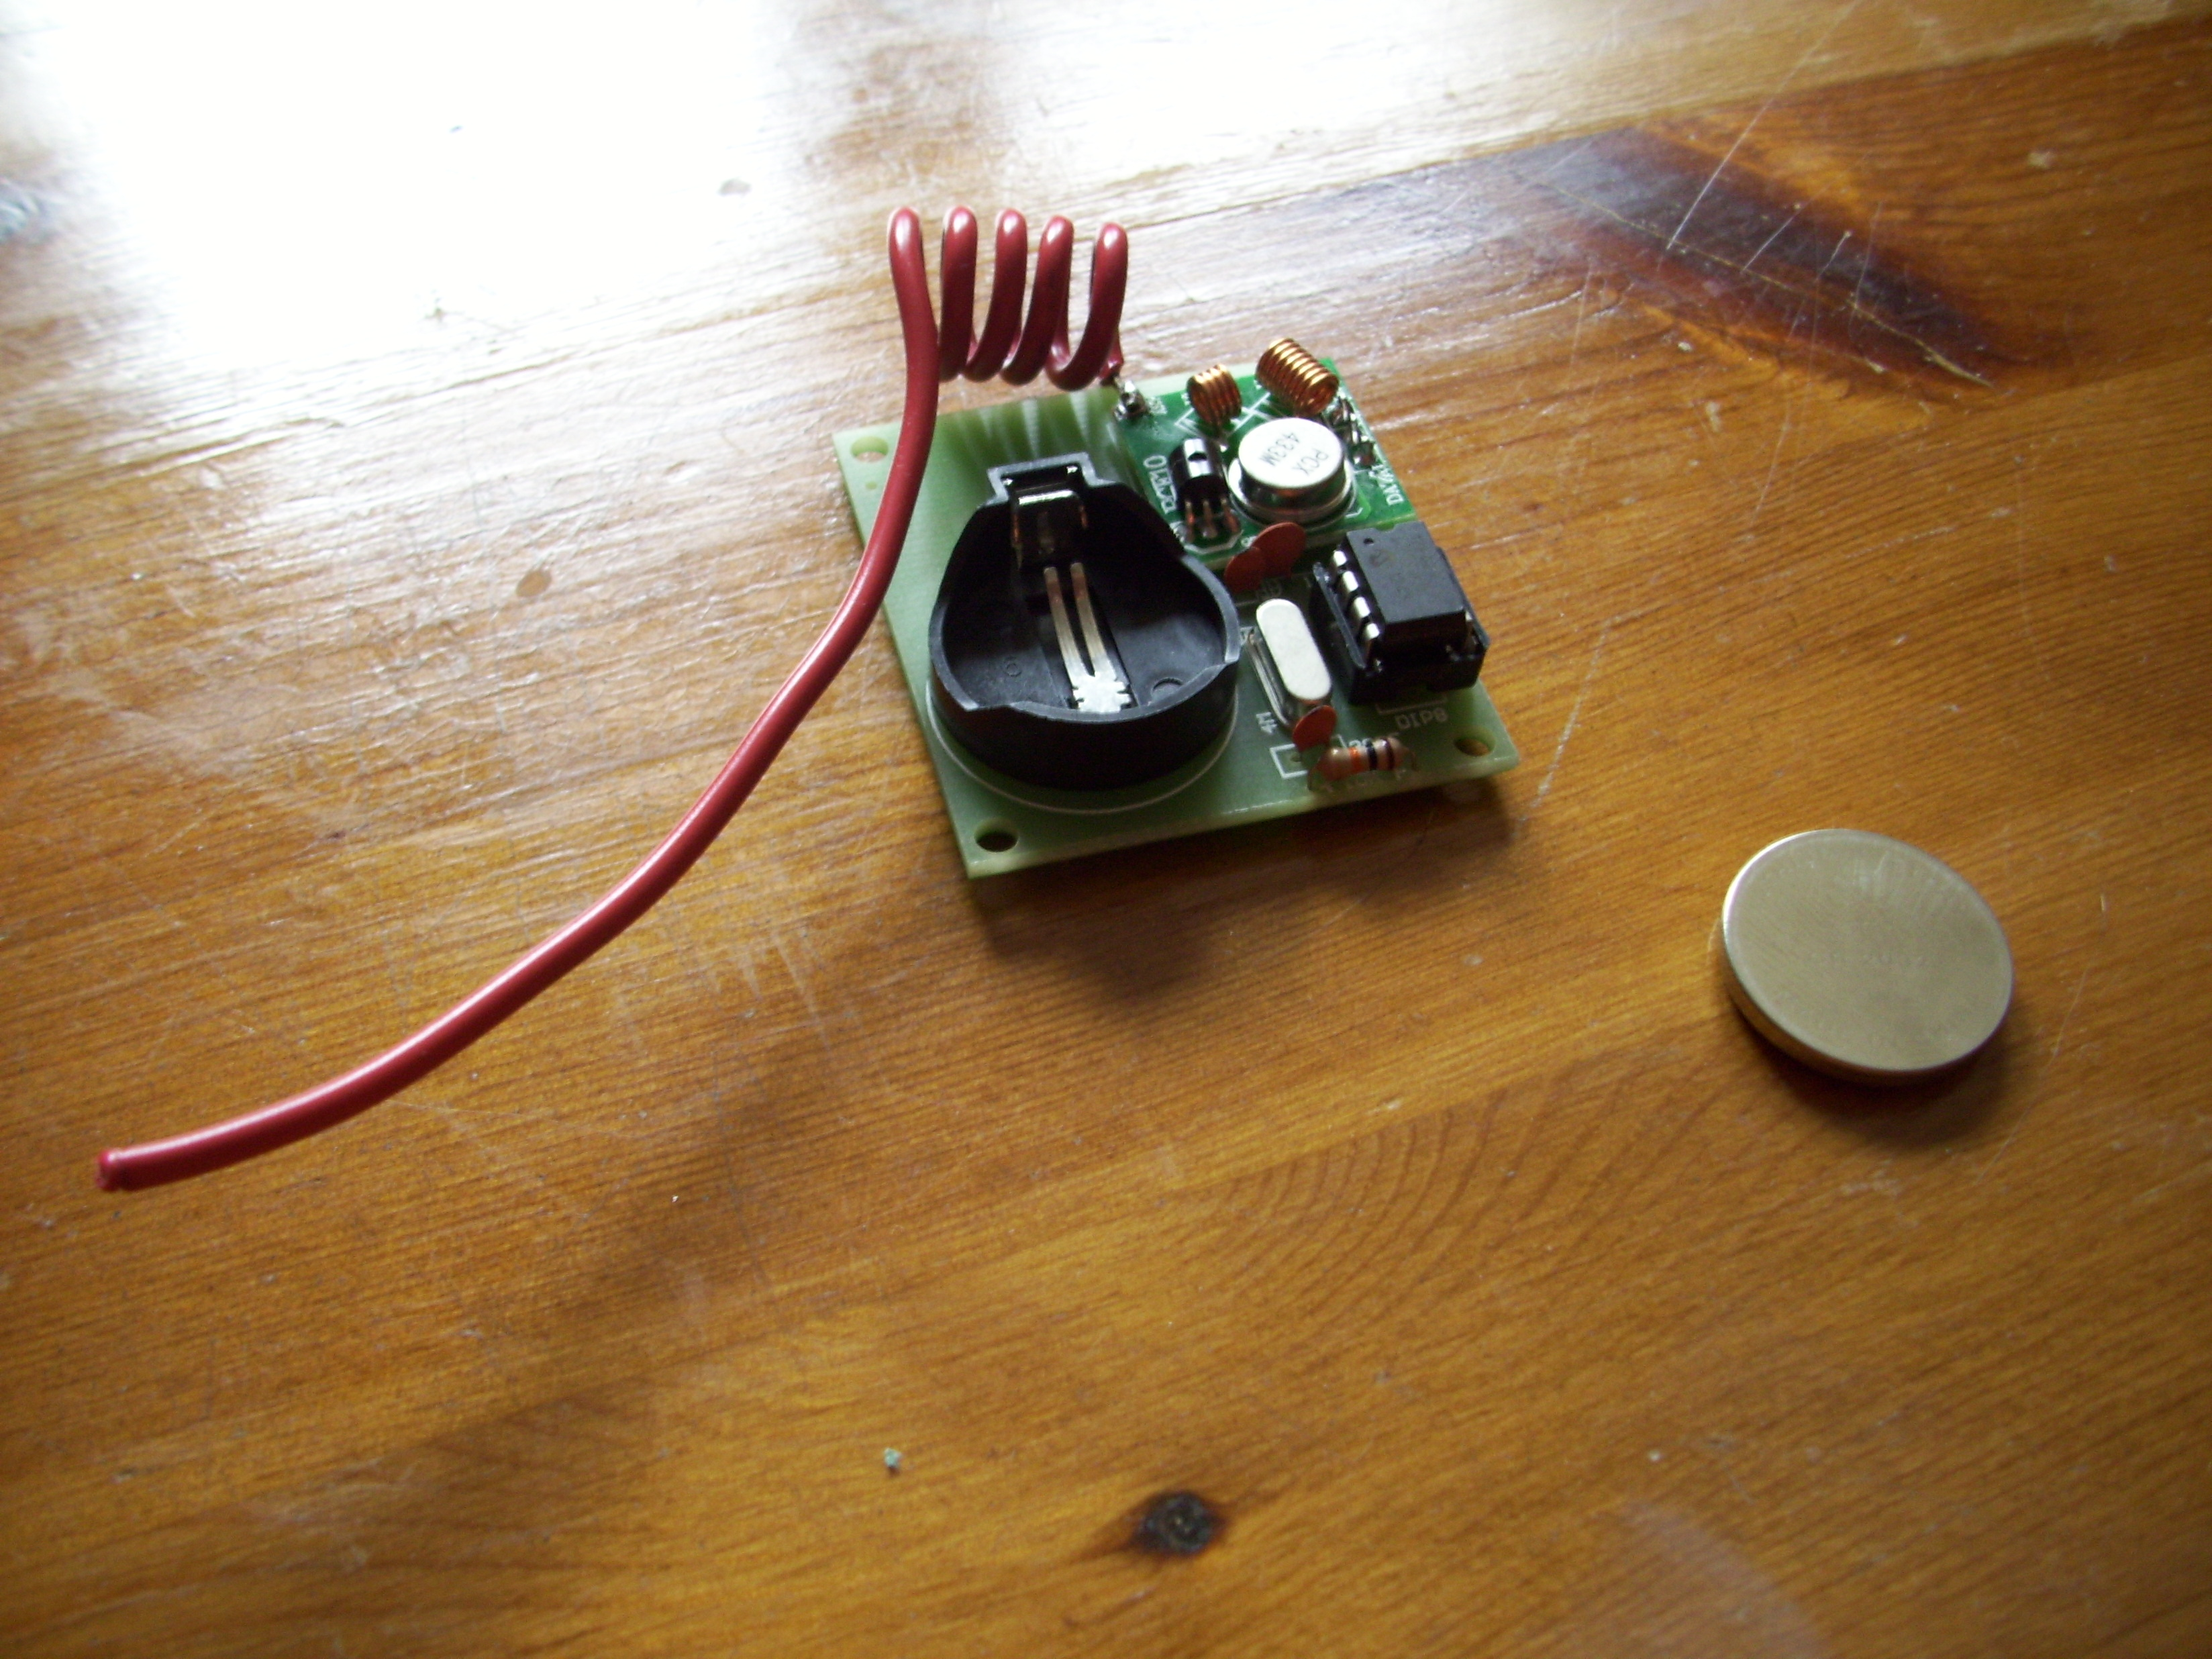
\includegraphics[width=\textwidth]{tag}
		\caption{One active RFID tag}
	\end{subfigure}
	\begin{subfigure}[b]{0.2\textwidth}
		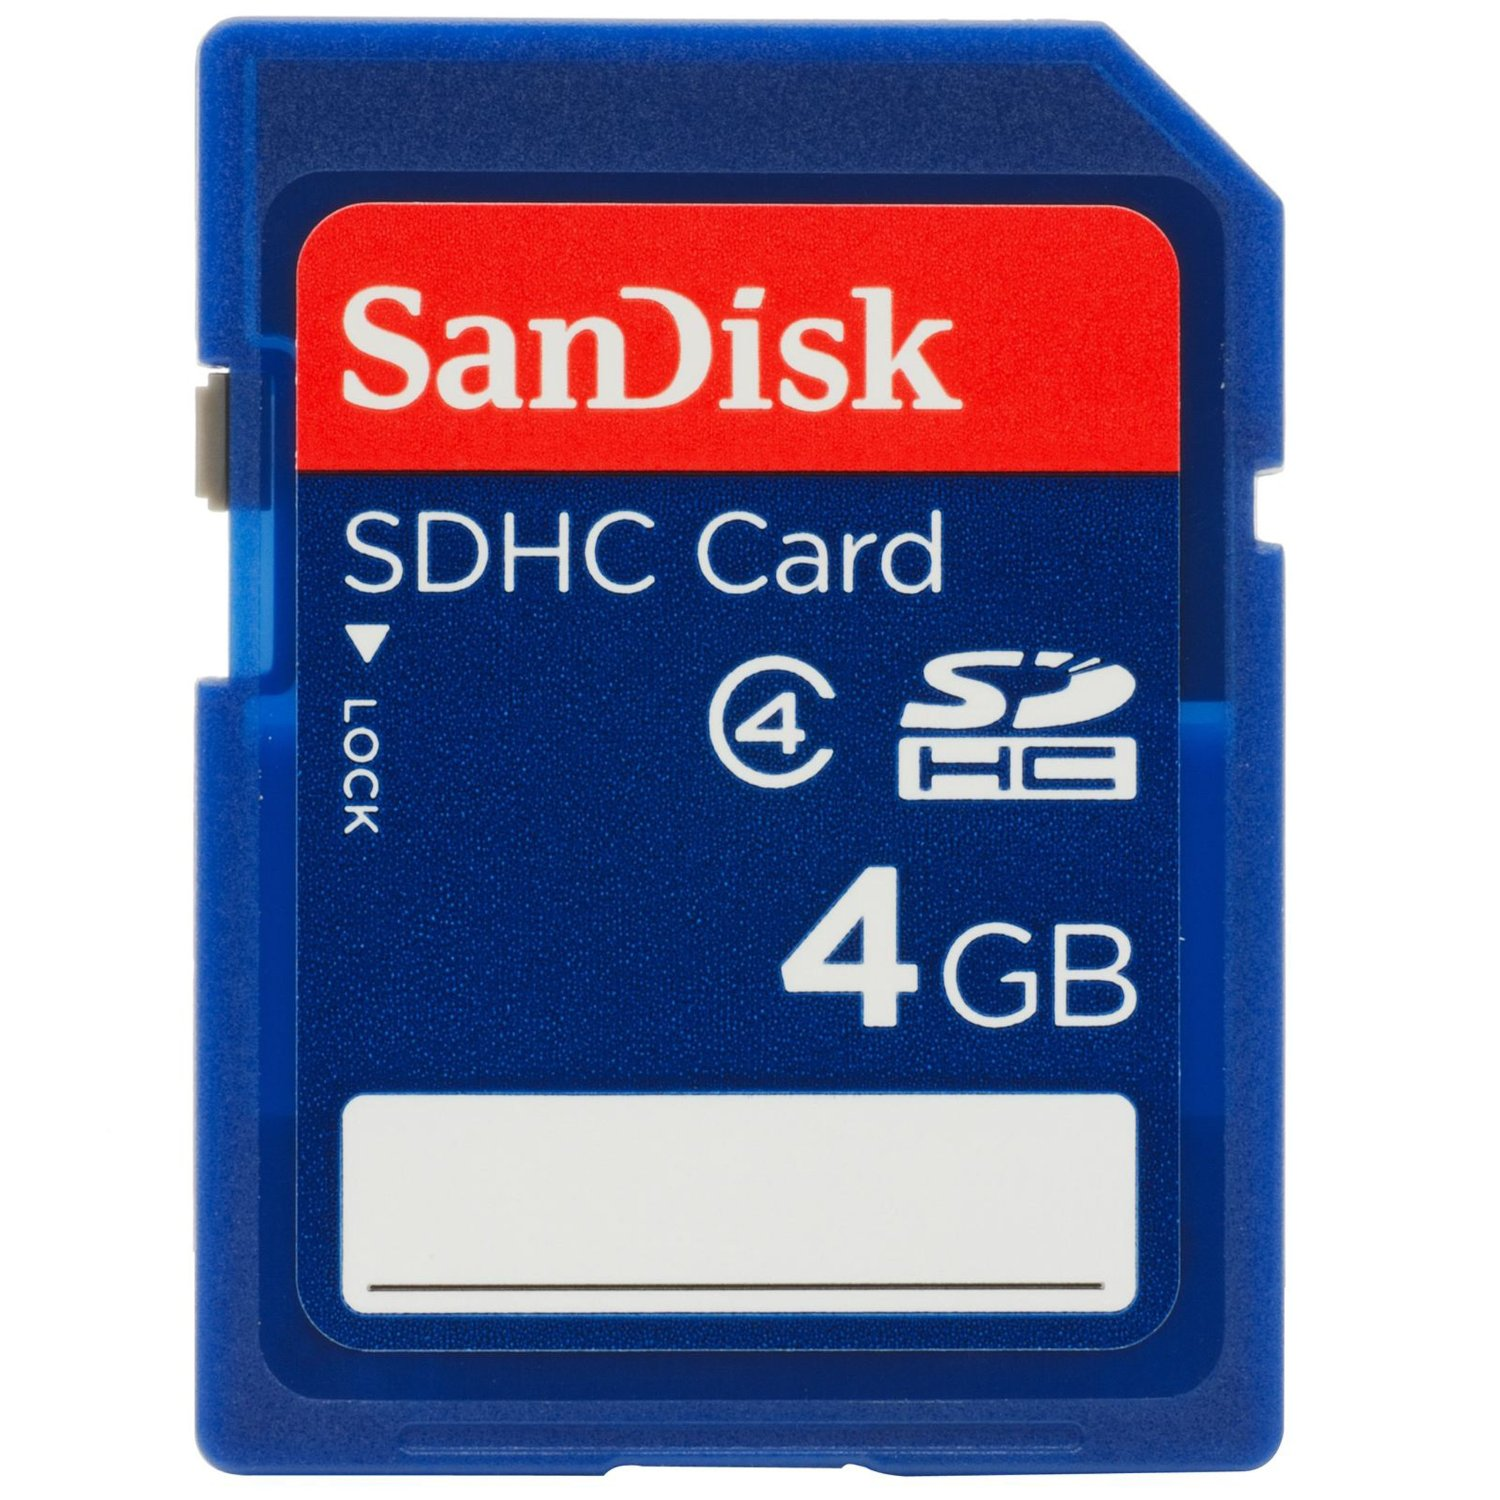
\includegraphics[width=\textwidth]{sdcard}
		\caption{SD card}
	\end{subfigure}
	\begin{subfigure}[b]{0.2\textwidth}
		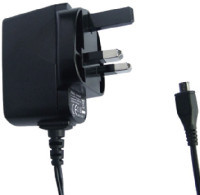
\includegraphics[width=\textwidth]{powersupply}
		\caption{Power supply}
	\end{subfigure}
	\caption{Hardware.}
\end{figure}

\newpage
\section{Software}

\subsection{Operating System}

The current operating system installed on the SD cars of the Raspberry Pis is Raspbian Linux\footnote{Raspbian Linux website - \url{http://www.raspbian.org/}}. Follow this guide if you want to install another Linux distribution: \url{http://elinux.org/RPi_Easy_SD_Card_Setup}. The devices have a user named \textbf{pi}. The password for both user \textbf{pi} and \textbf{root} is \underline{rfid2013michael}.

\subsection{Hostnames and IP addresses}

The devices were renamed to \textbf{pi0}, \textbf{pi1}, and \textbf{pi2}. The Raspberry Pi computers, the SD cards, and the RFID readers were marked with numbers \textbf{0}, \textbf{1}, and \textbf{2}.

The devices have static IP addresses assigned for their wired network interfaces. The IP addresses that were chosen are \textbf{192.168.1.10}, \textbf{192.168.1.11}, and \textbf{192.168.1.12}. These can be changed in \verb!/etc/network/interfaces! under root.

\begin{lstlisting}[caption=The interfaces file of \textbf{pi2}]
auto lo

iface lo inet loopback

auto eth0
iface eth0 inet static
address 192.168.1.12
netmask 255.255.255.0
broadcast 192.168.1.254
gateway 192.168.1.1

allow-hotplug wlan0
iface wlan0 inet manual
wpa-roam /etc/wpa_supplicant/wpa_supplicant.conf
iface default inet dhcp
\end{lstlisting}

In addition, each computer can communicate with the others by name, which is defined in \verb!/etc/hosts!.

\begin{lstlisting}[caption=The hosts file of \textbf{pi2}]
127.0.0.1		localhost
::1				localhost ip6-localhost ip6-loopback
fe00::0			ip6-localnet
ff00::0			ip6-mcastprefix
ff02::1			ip6-allnodes
ff02::2			ip6-allrouters

127.0.1.1		pi2
192.168.1.10	pi0
192.168.1.11	pi1
\end{lstlisting}

\subsection{Web server}

\textsc{Apache} HTTP web server is running on \textbf{pi2} at \textbf{192.168.1.12}. It serves requests to display the web interface of the system. The website requires a password before it can be accessed. The username is \underline{michael} and the password is \underline{rfid2013}. All web files are located in \verb!/var/www/!. The web interface is written in \textsc{PHP}.

\subsection{Localisation System}

First, make sure the RFID readers are connected to the Raspberry Pi computers. Also, ensure the computers are connected in a computer network.Then, the system starts by typing "\verb!python main.py!" on the server Raspberry Pi computer \textbf{pi2}. Next, type "\verb!python network_client.py!" on \textbf{pi0} and \textbf{pi1}. On the server \textbf{pi2} you will see the others connecting to it. If the RFID tag has its battery plugged in, then the computers will start receiving RFID measurements. The server will aggregate these values, update the database, and pass them to the localisation algorithm. The results will be visualised on the web interface.

\newpage

\begin{table}[H]
	\centering
	\begin{tabular}{ | r || l | }
		\hline
		\textbf{Specification}	& \textbf{Value} \\ \hline
		Dimensions				& 8.6cm x 5.4cm \\ \hline
		Weight					& 45g \\ \hline
		Power source			& 5V MircroUSB or GPIO \\ \hline
		Power rating			& 700mA (3.5W) \\ \hline
		System on a chip		& Broadcom BCM2835 \\ \hline
		CPU						& 700MHz ARM1176JZF-S \\ \hline
		GPU						& Broadcom VideoCore IV 250MHz \\ \hline
		Memory					& 512MB \\ \hline
		Storage:				& SD card slot \\ \hline
		USB	2.0 ports			& 2 \\ \hline
		Networking				& 10/100 Ethernet \\ \hline
		Low-level peripherals	& 8 x GPIO, UART, I$^{2}$C bus, SPI bus \\ \hline
		Operating system		& Raspbian Linux \\ \hline
		Price					& US \textdollar 35 \\ \hline
	\end{tabular}
	\caption{Specifications of the Raspberry Pi Model B revision 2 single-board computer.}
\end{table}

\begin{table}[H]
	\centering
	\begin{tabular}{ | r || l | }
		\hline
		\textbf{Specification}	& \textbf{Value} \\ \hline
		Dimensions				& 4cm x 6cm x 1.8cm \\ \hline
		Operating Temperature	& 0 - 50$^\circ$ C	\\ \hline
		Operating Frequency		& 315 MHz	\\ \hline
		Incoming signal range	& 60 dBm \\ \hline
		Power source			& Serial / USB port, DC 9V socket \\ \hline
		Communication			& RS-232 serial port \\ \hline
		Watchdog timer			& 2.3 seconds \\ \hline
		Simultaneous reads		& 80 tags	\\ \hline
		Reader control			& No control protocol \\ \hline
		Data representation		& Raw character data, No data encryption	\\ \hline
		Data output				& ID: 4 characters + RSSI: 0-255 \\ \hline
		Price					& US \textdollar 49.95 \\ \hline
	\end{tabular}
	\caption{Specifications of RF9315R-u active RFID reader.}
\end{table}

\begin{table}[H]
	\centering
	\begin{tabular}{ | r || l | }
		\hline
		\textbf{Parameter}		& \textbf{Value} \\ \hline
		Baud rate				& 9600 bits per second \\ \hline
		Data bits				& 8 bits \\ \hline
		Stop bits				& 1 bit \\ \hline
		Parity					& None \\ \hline
		Flow control			& None \\ \hline
	\end{tabular}
	\caption{Serial port parameter settings to communicate with the readers.}
\end{table}

\begin{table}[H]
	\centering
	\begin{tabular}{ | r || l | }
		\hline
		\textbf{Specification}	& \textbf{Value} \\ \hline
		Dimensions				& 4cm x 5cm x 1.8cm \\ \hline
		Operating Temperature	& 0 - 50$^\circ$ C	\\ \hline
		Operating Frequency		& 315 MHz	\\ \hline
		Power source			& CR2025 / CR2032 battery \\ \hline
		Battery life			& 5,000 / 7,000 hours \\ \hline
		Power consumption		& 4mA when transmitting, 19uA when idle \\ \hline
		RF output power			& $<$ 2mW \\ \hline
		Effective range			& 8 meters with 8mm coil diameter, 2cm long antenna \\ \hline
		Data output				& ID: 4 characters \\ \hline
		Price					& US \textdollar 19.95 \\ \hline
	\end{tabular}
	\caption{Specifications of RF8315T active RFID tag.}
\end{table}

\end{document}
